\documentclass[11pt]{article}

\author{Dylan Toirkens, Joey Wilmots}
\title{\textbf{Taak 1: Studie van ontwerpprincipes van Shneiderman en Norman}}
\date{18/10/2017}

\usepackage{graphicx}
\usepackage{float}
\usepackage[dutch]{babel}


\setcounter{tocdepth}{3}
\setcounter{secnumdepth}{3}
\begin{document}
	\begin{titlepage}
		
		\newcommand{\HRule}{\rule{\linewidth}{0.5mm}} % Defines a new command for the horizontal lines, change thickness here
		
		\begin{center} % Center everything on the page
			
			\textsc{\LARGE Universiteit Hasselt}\\[1.5cm] % Nme of your university/college
			\textsc{\Large Humane en sociale aspecten van de informatica}\\[0.5cm] % Major heading such as course name
			
			\HRule \\[0.4cm]
			{ \huge \bfseries Taak 1: Studie van ontwerpprincipes van Shneiderman en Norman}\\[0.4cm]
			\HRule \\[1.5cm]
			
			\begin{minipage}{0.5\textwidth}
				\begin{flushleft} \large
					Groep 10:\newline
					Dylan \textsc{Toirkens}\newline
					Joey \textsc{Wilmots}
				\end{flushleft}
			\end{minipage}
			~
			\begin{minipage}{0.3\textwidth}
				\begin{flushright} \large
					\emph{Datum:}\\
					16 oktober 2017
					\emph{Academiejaar: } \\
					2017-2018
				\end{flushright}
			\end{minipage}\\[3cm]
			\vspace{25 mm}
			
\includegraphics[width=3.0cm]{UHasselt-logo.jpg}\\[2.0cm]  
		\end{center}
	\end{titlepage}
\newpage
\tableofcontents
\clearpage

\section{Inleiding}

\section{Bespreking Dylan}
Zowel Spotify als iTunes heb ik nog nooit gebruikt. Mijn bespreking over deze 2 applicaties zal dus gebaseerd zijn op de eerste indruk die ik heb bij het gebruik hiervan. Er was echter wel een beperking die ik ondervond bij het uitproberen van iTunes. Veel functionaliteit wordt pas beschikbaar gesteld nadat de gebruiker aangemeld is. Het aanmaken van een account kon ik niet voltooien, waardoor een aantal mogelijkheden van iTunes vergrendeld was voor mij. Hierdoor zal mijn besprekingen over iTunes ook gebaseerd zijn op de verwachtingen die ik heb wanneer ik iets probeer uit te voeren.
\subsection{Ontwerpprincipes van Shneiderman}
\subsubsection{Herken de diversiteit}
De belangrijkste functionaliteit van Spotify en iTunes is het voorzien van muziek aan de gebruiker. Met dit in gedachte kan ik de doelgroep indelen in 3 groepen: nieuwe gebruikers, gebruikers die de applicatie af en toe gebruiken en gebruikers die het vaak tot zelfs dagelijks gebruiken. 

\textbf{Nieuwe gebruikers} zouden de applicatie kunnen raadplegen voor het afspelen van een specifieke nummer, de radio of een vooropgemaakte afspeellijst, zoals een top 50 of nummers van een specifieke genre. Om een specifiek nummer af te spelen, zou er de mogelijkheid moeten zijn om te kunnen zoeken naar het nummer op vlak van een zoekcriteria. Beide applicaties doen dit in de vorm van een zoekbalk, zoals te zien is in Figuur \ref{fig:SZoek} voor Spotify. Tijdens het ingeven van een zoekterm geven beide applicaties al mogelijke aanvulsuggesties, wat ik zeker iets positiefs vind voor nieuwe gebruikers. Wanneer een nummer gekozen is, verschijnt de titel, artiest en album op het scherm. Om naar de radio te luisteren, dient er voor beide programma's genavigeerd te worden naar \textquotedblleft Radio\textquotedblright en kan er vervolgens een aangeboden station gekozen worden. Het raadplegen van vooropgestelde afspeellijsten wordt door beide applicaties in ongeveer evenveel stappen gedaan, maar wordt wel anders aangegeven. In Spotify dient er eerst op \textquotedblleft Bladeren\textquotedblright geklikt te worden, vervolgens kan er eventueel een tabblad gekozen worden om het aanbod te specifi\"{e}ren en dan kan een afspeellijst gekozen worden. In iTunes klikt de gebruiker eerst op \textquotedblleft Ontdekken\textquotedblright, kiest dan het tabblad \textquotedblleft Afspeellijsten\textquotedblright en vervolgens eventueel een genre, activiteit of sfeer. Deze 3 stappen worden weergegeven in Figuur \ref{fig:IAfspeellijst}. Nu kan de gebruiker een afspeellijst kiezen. We zien dat de gebruiker slechts weinig acties hoeft uit te voeren om muziek af te kunnen spelen bij beide applicaties. Er wordt ook duidelijke feedback gegeven over het nummer dat afgespeeld wordt. Dit helpt nieuwe gebruikers zeker op weg.

\textbf{Gebruikers die de applicatie af en toe gebruiken} kunnen nood hebben aan het opslaan van nummers in een eigen bibliotheek. Nadat een aantal nummers in de bibliotheek toegevoegd is, kan een persoonlijke afspeellijst aangemaakt worden. In beide applicaties is dit mogelijk.

\textbf{Gebruikers die het vaak tot zelfs dagelijks gebruiken} hebben de mogelijkheid om nummers in een wachtrij te zetten, afspeellijsten te importenen en te generen.
\begin{figure}
	\centering
	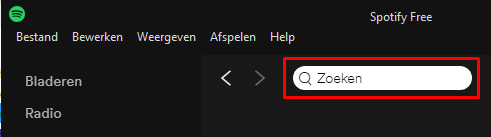
\includegraphics[width=0.9\textwidth]{SZoek.png}
	\caption{Zoekbalk in Spotify.}
	\label{fig:SZoek}
\end{figure}
\begin{figure}
	\centering
	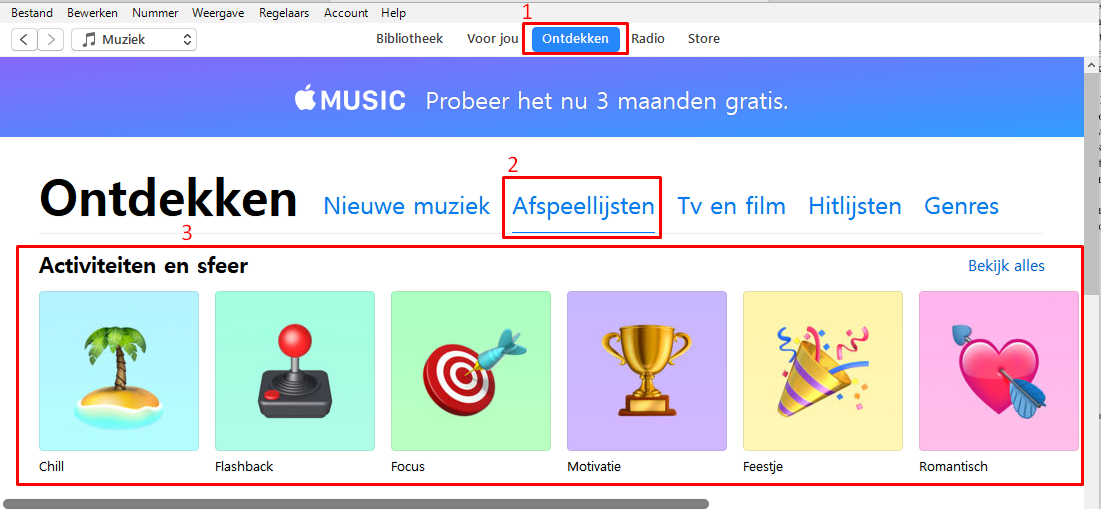
\includegraphics[width=0.9\textwidth]{IAfspeellijst.png}
	\caption{Het raadplegen van een vooropgemaakte afspeellijst in iTunes kan bereikt worden door de aangeduide stappen in volgorde te doen.}
	\label{fig:IAfspeellijst}
\end{figure}
\subsubsection{De acht gouden regels voor interface design}
\begin{itemize}
	\item Streven naar consistentie\\
	In de meeste programma's is een menubalk aanwezig waar de veel gebruikte functies in terug te vinden is. Als deze consistent t.o.v. andere applicaties ingedeeld is, kan een gebruiker vlotter de handeling terugvinden die ze zoekt. In Figuur \ref{fig:SMenubalk} en \ref{fig:IMenubalk} zijn de menubalken van respectievelijk Spotify en iTunes te zien. De gemeenschappelijke items zijn \textquotedblleft Bestand\textquotedblright, \textquotedblleft Bewerken\textquotedblright, \textquotedblleft Weergeven\textquotedblright en \textquotedblleft Help\textquotedblright. Deze komen ook in dezelfde volgorde voor, met eventueel andere items daartussen ingevoegd. Een ander voorbeeld van een goed gebruik van consistentie is dat de tabbladen op verschillende pagina's steeds op dezelfde plaats staan. In Figuur \ref{fig:ITabs} is een voorbeeld te zien voor iTunes, waarbij de tabbladen van \textquotedblleft Ontdekken\textquotedblright en \textquotedblleft Radio\textquotedblright op dezelfde plaats terug te vinden zijn. De \textquotedblleft Store\textquotedblright van iTunes is echter zonder tabbladen ingedeeld, zoals te zien is in Figuur \ref{fig:IStore}. Dit is dus niet consistent met de indeling die te vinden is bij \textquotedblleft Ontdekken\textquotedblright en \textquotedblleft Radio\textquotedblright.
	\begin{figure}
		\centering
		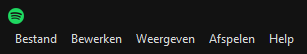
\includegraphics[width=0.9\textwidth]{SMenubalk.png}
		\caption{Menubalk van Spotify.}
		\label{fig:SMenubalk}
	\end{figure}
	\begin{figure}
	\centering
	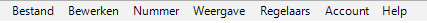
\includegraphics[width=0.9\textwidth]{IMenubalk.png}
	\caption{Menubalk van iTunes.}
	\label{fig:IMenubalk}
	\end{figure}
	\begin{figure}
	\centering
	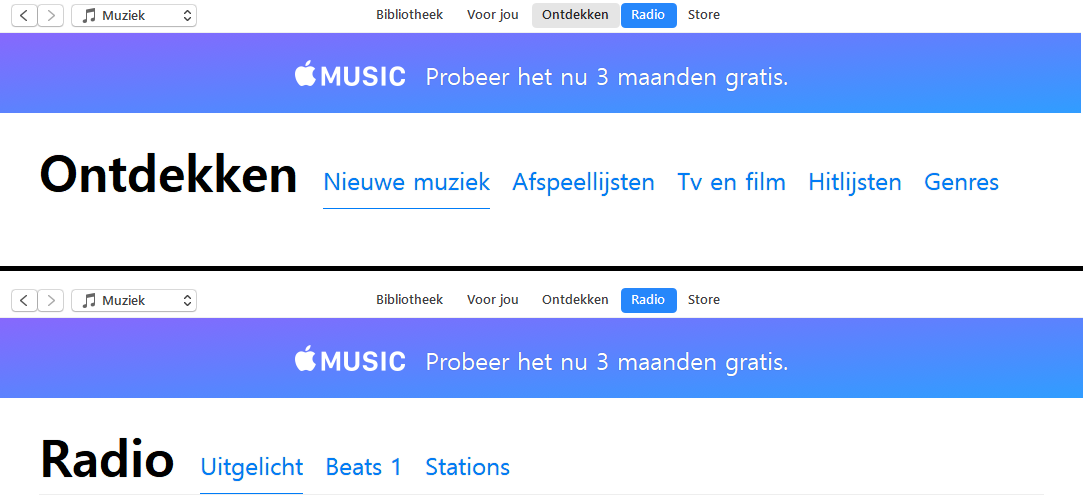
\includegraphics[width=0.9\textwidth]{ITabs.png}
	\caption{De tabbladen staan op dezelfde plaats zoals te zien bij \textquotedblleft Ontdekken\textquotedblright (boven) en \textquotedblleft Radio\textquotedblright (onder).}
	\label{fig:ITabs}
	\end{figure}
	\begin{figure}
	\centering
	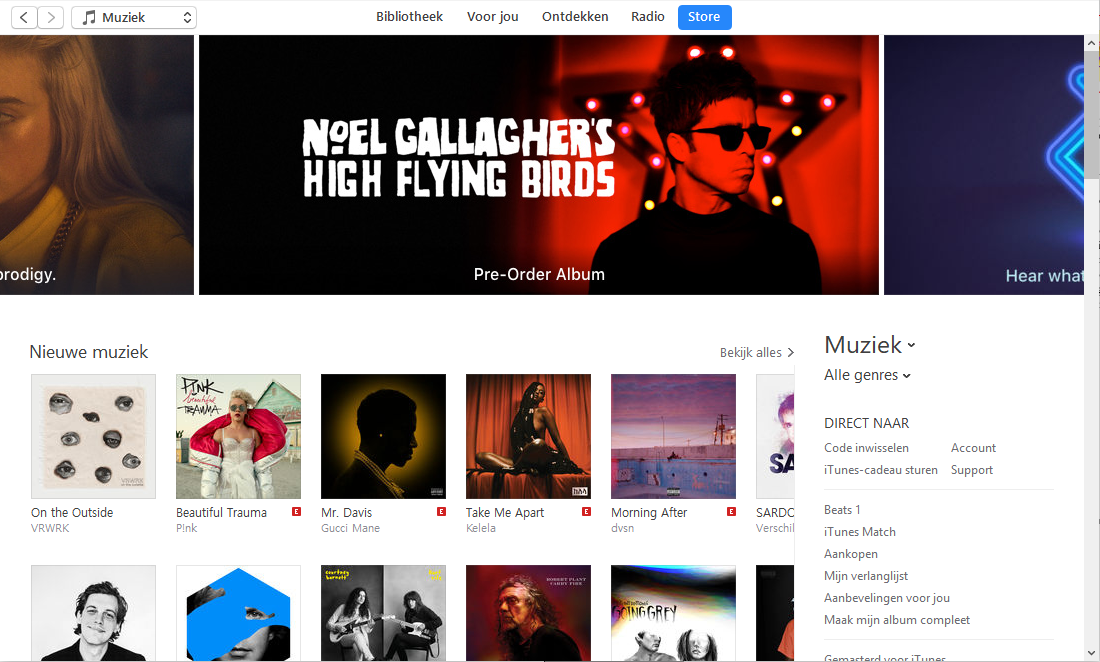
\includegraphics[width=0.9\textwidth]{IStore.png}
	\caption{De \textquotedblleft Store\textquotedblright van iTunes maakt geen gebruik van tabbladen, wat niet consistent is met \textquotedblleft Ontdekken\textquotedblright en \textquotedblleft Radio\textquotedblright.}
	\label{fig:IStore}
	\end{figure}
	\item Frequente gebruikers toelaten shortcuts te gebruiken\\
	In Spotify kan een gebruiker een nummer dat afgespeeld wordt toevoegen opslaan in de bibliotheek door te klikken op het plussymbool dat te vinden is naast de titel van het nummer. Dit is te zien in Figuur \ref{fig:SOpslaan}. Dit is een shortcut t.o.v. het toevoegen van een nummer d.m.v. het gebruik van de menu dat geopend wordt wanneer er met de rechtermuisknop geklikt wordt op een nummer.
	\begin{figure}
		\centering
		
\includegraphics[width=0.9\textwidth]{SOpslaan.png}
		\caption{De gebruiker kan met 1 klik op het plussymbool het nummer dat afgespeeld wordt opslaan in de bibliotheek.}
		\label{fig:SOpslaan}
	\end{figure}
	\item Informatie feedback bieden\\
	Beide applicaties tonen het nummer dat op dit moment afgespeeld wordt samen met de arties en de cover van het album. Ook wordt de tijdsduur van het nummer getoond en de voortgang in het nummer, zoals te zien is in Figuur \ref{fig:SFeedback}. Het was voor mij echter niet mogelijk te weten of een nummer toegevoegd werd aan de wachtlijst en om de lijst van nummers te tonen die in de wachtlijst staan. Dit is een minpunt op vlak van feedback. Dit zou opgelost kunnen worden door een popup bericht te geven wanneer een nummer in de wachtrij toegevoegd wordt. De wachtij raadplegen zou gedaan kunnen worden bij het raadplegen van een afspeellijst, waarbij de wachtrij zogezegd een tijdelijke afspeellijst is.
	\begin{figure}
		\centering
		
\includegraphics[width=0.9\textwidth]{SFeedback.png}
		\caption{De titel, arties en cover van het album van het nummer dat afgespeeld wordt, worden bij elkaar weergegeven. Daarnaast wordt ook de voortgang in het nummer getoond.}
		\label{fig:SFeedback}
	\end{figure}
	\item Dialogen ontwerpen zodat onverwachte resultaten uitgesloten worden en de voortgang duidelijk is\\
	Wanneer de gebruiker een nieuwe AppleID aanmaakt in iTunes, wordt dit mogelijk gemaakt aan de hand van een dialoog. Hierdoor kan de gebruiker de registratie uitvoeren zonder veel misverstanden. De velden worden gecontroleerd voordat er naar het volgende scherm genavigeerd wordt. De voortgang wordt echter niet weergegeven. Dit is te zien in Figuur \ref{fig:IAppleID}.
	\begin{figure}
		\centering
		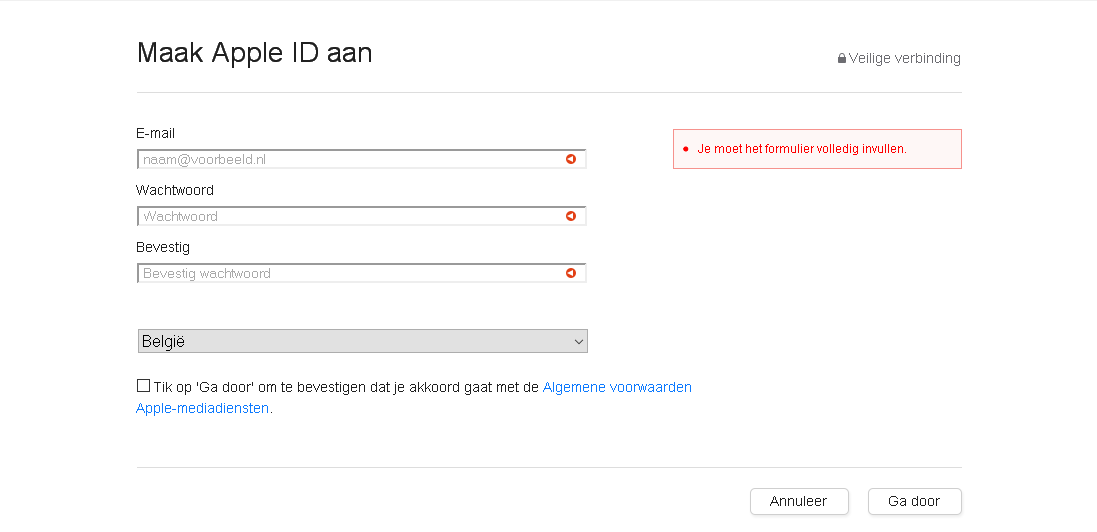
\includegraphics[width=0.9\textwidth]{IAppleID.png}
		\caption{De dialog die getoond wordt bij het aanmaken van een AppleID in iTunes.}
		\label{fig:IAppleID}
	\end{figure}
	\item Aandacht hebben voor foutenpreventie en op een eenvoudige manier fouten afhandelen\\
	Wanneer de gebruiker naar het volgende scherm probeert te gaan bij het aanmaken van een AppleID terwijl een veld nog leeg is, wordt ieder veld dat niet ingevuld is gemarkeerd en komt er een melding, zoals te zien in Figuur \ref{fig:IAppleID}. Er kan ook een popup komen, wat het geval is als de gebruiker nog niet aangevinkt heeft dat deze akkoord gaat met de algemene voorwaarden Apple-mediadiensten. Dit is te zien in Figuur \ref{fig:IAppleIDAkkoord}.
	\begin{figure}
		\centering
		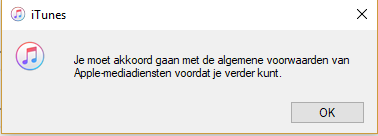
\includegraphics[width=0.9\textwidth]{IAppleIDAkkoord.png}
		\caption{Een popup verschijnt wanneer de gebruiker verder probeert te gaan zonder de voorwaarden te accepteren.}
		\label{fig:IAppleIDAkkoord}
	\end{figure}
	\item Acties omkeerbaar maken\\
	In beide applicaties kan de gebruiker ervoor kiezen om het huidige nummer over te slaan en het volgende nummer af te spelen. Mocht dit niet gewenst zijn, kan er toch nog terug genavigeerd worden.
	\item De gebruiker meester over het systeem laten zijn\\
	In Spotify kan een nieuw nummer gekozen automatisch gekozen worden wanneer een nummer voorbij is. Als dit niet gewenst is, kan de gebruiker dit in de instellingen uitschakelen, zoals te zien is in Figuur \ref{fig:SAutoplay}
	\begin{figure}
		\centering
		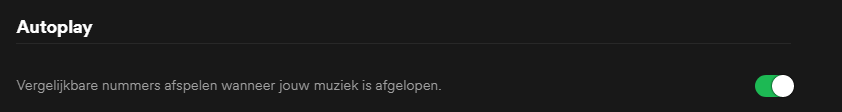
\includegraphics[width=0.9\textwidth]{SAutoplay.png}
		\caption{De gebruiker kan het automatisch afspelen van nummers uitschakelen in de instellingen.}
		\label{fig:SAutoplay}
	\end{figure}
	\item Het aantal gegevens beperken dat de gebruiker op korte termijn moet onthouden\\
	Naar mijn mening zijn er steeds niet veel stappen die de gebruiker moet onthouden om een handeling uit te voeren. Dit is dus al in orde voor beide applicaties.
\end{itemize}
\subsection{Ontwerpprincipes van Norman}
\subsubsection{Visibility}
De belangrijkste tabbladen zijn duidelijk en altijd terug te vinden op iedere pagina. In Spotify staan ze links en in iTunes staan ze boven. Knoppen om het nummer dat afgespeeld wordt in de afspeellijst te manipuleren zijn ook bij elkaar te vinden. In Spotify zien de knoppen eruit zoals in Figuur \ref{fig:SFeedback}.
\subsubsection{Affordances}
Er zijn weinig voorbeelden van affordance te vinden in beide applicaties. Het is mogelijk om te navigeren in een nummer door een bolletje te verschuiven over een balk, zoals te zien is in Figuur \ref{fig:SScrolbalk}. In Spotify wordt dit bolletje echter pas weergeven wanneer de gebruiker met de cursor over deze balk staat. Dit is dus geen goede visibiltiy voor deze funcionaliteit, maar de affordance dat je het bolletje kan verschuiven vind ik wel in orde.
\begin{figure}
	\centering
	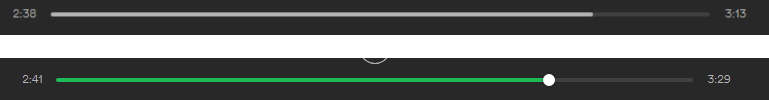
\includegraphics[width=0.9\linewidth]{SScrolbalk.png}
	\caption{Het bolletje dat kan gebruikt worden om te navigeren in een nummer in Spotify wordt pas zichtbaar als de cursor boven de balk staat.}
	\label{fig:SScrolbalk}
\end{figure}
\subsubsection{Mappings}
De knoppen om naar het volgende nummer te navigeren staat rechts van de knop om naar het vorig nummer te navigeren, zoals te zien in Figuur \ref{fig:SFeedback}. Dit is een goede mapping omdat de denkwijze ook is dat iets wat links staat, voor iets wat rechts staat is.
\subsubsection{Feedback}
Wanneer een nummer afgespeeld wordt, wordt informatie weergegeven zoals in Figuur \ref{fig:SFeedback} (visuele feedback) en kan de gebruiker natuurlijk horen of het afgespeeld wordt (auditieve feedback). Een ander voorbeeld is dat wanneer het volume naar het minimaal gebracht wordt, dan het symbool veranderd naar een microfoon met een kruisje, zoals te zien in Figuur \ref{fig:SVolumeOff}
\begin{figure}
	\centering
	
\includegraphics[width=0.5\linewidth]{SVolumeOff}
	\caption{Er komt een kruisje te staan bij het symbool voor volume wanneer het volume uit staat.}
	\label{fig:SVolumeOff}
\end{figure}
\subsubsection{Constraints}
Bij het aanmaken van een AppleID moet een e-mailadres een correcte formaat hebben. De gebruiker kan dus niet verder gaan als deze niet correct is, zoals te zien is in Figuur \ref{fig:IEmail}.
\begin{figure}
	\centering
	
\includegraphics[width=0.9\linewidth]{IEmail}
	\caption{De gebruiker kan niet naar het volgende scherm gaan als het e-mailadres niet in het juiste formaat is.}
	\label{fig:IEmail}
\end{figure}

\section{Bespreking Joey}

\section{Conclusie}

\end{document}

